% !TeX encoding = UTF-8
% !TeX program = xelatex
% !TeX spellcheck = en_US

\documentclass[degree=master, degree-type=professional, fontset=fandol]{thuthesis}
  % 学位 degree:
  %   doctor | master | bachelor | postdoc
  % 学位类型 degree-type:
  %   academic(默认)| professional


% 论文基本配置,加载宏包等全局配置
% !TeX root = ./thuthesis-example.tex

% 论文基本信息配置

\thusetup{
  %******************************
  % 注意:
  %   1. 配置里面不要出现空行
  %   2. 不需要的配置信息可以删除
  %   3. 建议先阅读文档中所有关于选项的说明
  %******************************
  %
  % 输出格式
  %   选择打印版(print)或用于提交的电子版(electronic),前者会插入空白页以便直接双面打印
  %
  output = print,
  %
  % 标题
  %   可使用“\\”命令手动控制换行
  %
  title  = {广领域与主动领域适应},
  title* = {Universal and Active Domain Adaptation},
  %
  % 学位
  %   1. 学术型
  %      - 中文
  %        需注明所属的学科门类,例如:
  %        哲学、经济学、法学、教育学、文学、历史学、理学、工学、农学、医学、
  %        军事学、管理学、艺术学
  %      - 英文
  %        博士:Doctor of Philosophy
  %        硕士:
  %          哲学、文学、历史学、法学、教育学、艺术学门类,公共管理学科
  %          填写“Master of Arts“,其它填写“Master of Science”
  %   2. 专业型
  %      直接填写专业学位的名称,例如:
  %      教育博士、工程硕士等
  %      Doctor of Education, Master of Engineering
  %   3. 本科生不需要填写
  %
  degree-name  = {工程硕士},
  degree-name* = {Master of Engineering},
  %
  % 培养单位
  %   填写所属院系的全名
  %
  department = {软件学院},
  %
  % 学科
  %   1. 学术型学位
  %      获得一级学科授权的学科填写一级学科名称,其他填写二级学科名称
  %   2. 工程硕士
  %      工程领域名称
  %   3. 其他专业型学位
  %      不填写此项
  %   4. 本科生填写专业名称,第二学位论文需标注“(第二学位)”
  %
  discipline  = {软件工程},
  discipline* = {Software Engineering},
  %
  % 姓名
  %
  author  = {付博},
  author* = {Bo Fu},
  %
  % 指导教师
  %   中文姓名和职称之间以英文逗号“,”分开,下同
  %
  supervisor  = {王建民, 教授},
  supervisor* = {Professor Jianmin Wang},
  %
  % 副指导教师
  %
  associate-supervisor  = {龙明盛, 副教授},
  associate-supervisor* = {Associate Professor Mingsheng Long},
  %
  % 联合指导教师
  %
  % joint-supervisor  = {某某某, 教授},
  % joint-supervisor* = {Professor Mou Moumou},
  %
  % 日期
  %   使用 ISO 格式;默认为当前时间
  %
  % date = {2019-07-07},
  %
  % 是否在中文封面后的空白页生成书脊(默认 false)
  %
  include-spine = false,
  %
  % 密级和年限
  %   秘密, 机密, 绝密
  %
  % secret-level = {秘密},
  % secret-year  = {10},
  %
  % 博士后专有部分
  %
  % clc                = {分类号},
  % udc                = {UDC},
  % id                 = {编号},
  % discipline-level-1 = {计算机科学与技术},  % 流动站(一级学科)名称
  % discipline-level-2 = {系统结构},          % 专业(二级学科)名称
  % start-date         = {2011-07-01},        % 研究工作起始时间
}

% 载入所需的宏包

% 可以使用 nomencl 生成符号和缩略语说明
% \usepackage{nomencl}
% \makenomenclature

% 表格加脚注
\usepackage{threeparttable}

% 表格中支持跨行
\usepackage{multirow}

% 固定宽度的表格。放在 hyperref 之前的话,tabularx 里的 footnote 显示不出来。
% \usepackage{tabularx}

% 跨页表格
% \usepackage{longtable}

% 量和单位
\usepackage{siunitx}

% 定理类环境宏包
\usepackage{amsthm}
% 也可以使用 ntheorem
% \usepackage[amsmath,thmmarks,hyperref]{ntheorem}

% 参考文献使用 BibTeX + natbib 宏包
% 顺序编码制
\usepackage[sort]{natbib}
\bibliographystyle{thuthesis-numeric}

% 著者-出版年制
% \usepackage{natbib}
% \bibliographystyle{thuthesis-author-year}

% 本科生参考文献的著录格式
% \usepackage[sort]{natbib}
% \bibliographystyle{thuthesis-bachelor}

% 参考文献使用 BibLaTeX 宏包
% \usepackage[backend=biber,style=thuthesis-numeric]{biblatex}
% \usepackage[backend=biber,style=thuthesis-author-year]{biblatex}
% \usepackage[backend=biber,style=apa]{biblatex}
% \usepackage[backend=biber,style=mla-new]{biblatex}
% 声明 BibLaTeX 的数据库
% \addbibresource{ref/refs.bib}

% 定义所有的图片文件在 figures 子目录下
\graphicspath{{figures/}}

% 数学命令
\newcommand\dif{\mathop{}\!\mathrm{d}}  % 微分符号

% hyperref 宏包在最后调用
\usepackage{hyperref}



\begin{document}

% 封面
\maketitle

% 学位论文指导小组、公开评阅人和答辩委员会名单
% !TeX root = ../thuthesis-example.tex

\begin{committee}[name={学位论文指导小组、公开评阅人和答辩委员会名单}]

  \newcolumntype{C}[1]{@{}>{\centering\arraybackslash}p{#1}}

  \section*{指导小组名单}

  \begin{center}
    \begin{tabular}{C{3cm}C{3cm}C{9cm}@{}}
      李XX & 教授     & 清华大学 \\
      王XX & 副教授   & 清华大学 \\
      张XX & 助理教授 & 清华大学 \\
    \end{tabular}
  \end{center}


  \section*{公开评阅人名单}

  \begin{center}
    \begin{tabular}{C{3cm}C{3cm}C{9cm}@{}}
      刘XX & 教授   & 清华大学                    \\
      陈XX & 副教授 & XXXX大学                    \\
      杨XX & 研究员 & 中国XXXX科学院XXXXXXX研究所 \\
    \end{tabular}
  \end{center}


  \section*{答辩委员会名单}

  \begin{center}
    \begin{tabular}{C{2.75cm}C{2.98cm}C{4.63cm}C{4.63cm}@{}}
      主席 & 赵XX                  & 教授                    & 清华大学       \\
      委员 & 刘XX                  & 教授                    & 清华大学       \\
          & \multirow{2}{*}{杨XX} & \multirow{2}{*}{研究员} & 中国XXXX科学院 \\
          &                       &                         & XXXXXXX研究所  \\
          & 黄XX                  & 教授                    & XXXX大学       \\
          & 周XX                  & 副教授                  & XXXX大学       \\
      秘书 & 吴XX                  & 助理研究员              & 清华大学       \\
    \end{tabular}
  \end{center}

\end{committee}



% 也可以导入 Word 版转的 PDF 文件
% \begin{committee}[file=figures/committee.pdf]
% \end{committee}


% 使用授权的说明
\copyrightpage
% 将签字扫描后授权文件 scan-copyright.pdf 替换原始页面
% \copyrightpage[file=scan-copyright.pdf]

\frontmatter
% !TeX root = ../thuthesis-example.tex

% 中英文摘要和关键字

\begin{abstract}
  论文的摘要是对论文研究内容和成果的高度概括。
  摘要应对论文所研究的问题及其研究目的进行描述,对研究方法和过程进行简单介绍,对研究成果和所得结论进行概括。
  摘要应具有独立性和自明性,其内容应包含与论文全文同等量的主要信息。
  使读者即使不阅读全文,通过摘要就能了解论文的总体内容和主要成果。

  论文摘要的书写应力求精确、简明。
  切忌写成对论文书写内容进行提要的形式,尤其要避免“第 1 章……;第 2 章……;……”这种或类似的陈述方式。

  关键词是为了文献标引工作、用以表示全文主要内容信息的单词或术语。
  关键词不超过 5 个,每个关键词中间用分号分隔。

  % 关键词用“英文逗号”分隔,输出时会自动处理为正确的分隔符
  \thusetup{
    keywords = {关键词 1, 关键词 2, 关键词 3, 关键词 4, 关键词 5},
  }
\end{abstract}

\begin{abstract*}
  An abstract of a dissertation is a summary and extraction of research work and contributions.
  Included in an abstract should be description of research topic and research objective, brief introduction to methodology and research process, and summarization of conclusion and contributions of the research.
  An abstract should be characterized by independence and clarity and carry identical information with the dissertation.
  It should be such that the general idea and major contributions of the dissertation are conveyed without reading the dissertation.

  An abstract should be concise and to the point.
  It is a misunderstanding to make an abstract an outline of the dissertation and words “the first chapter”, “the second chapter” and the like should be avoided in the abstract.

  Keywords are terms used in a dissertation for indexing, reflecting core information of the dissertation.
  An abstract may contain a maximum of 5 keywords, with semi-colons used in between to separate one another.

  % Use comma as seperator when inputting
  \thusetup{
    keywords* = {keyword 1, keyword 2, keyword 3, keyword 4, keyword 5},
  }
\end{abstract*}


% 目录
\tableofcontents

% 插图和附表清单
\listoffiguresandtables  % 插图和附表清单
% \listoffigures           % 插图清单
% \listoftables            % 附表清单

% 符号对照表
% !TeX root = ../thuthesis-example.tex

\begin{denotation}[3cm]
\item[CNN]	卷积神经网络 (Convolutional Neural Networks)
\item[DA]	领域适应 (Domain Adaptation)
\item[DANN]	领域对抗神经网络 (Domain Adversarial Neural Network)
\item[GRL]	梯度反转层 (Gradient Reversal Layer)
\item[CDAN]	条件对抗领域适应 (Conditional Adversarial Domain Adaptation)
\item[FGVC]	细粒度视觉识别 (Fine-Grained Visual Recognition)
\item[$\mathcal{S}$]	迁移学习源领域
\item[$n_{\mathcal{S}}$]	源领域$\mathcal{S}$上的样本数量
\item[$\mathcal{T}$]	迁移学习目标领域
\item[$n_{\mathcal{T}}$]	 目标领域$\mathcal{T}$上的样本数量
\item[$y_c^k|_{k=1}^K$]	样本$x$的$K$个粗粒度类别标记
\item[$d$]	样本$x$的领域类别标记
\item[$\rm D$]	领域判别器
\item[$L_c$]	交叉熵损失函数
\item[$D_{KL}$]		 KL散度函数

\end{denotation}



% 也可以使用 nomencl 宏包,需要在导言区
% \usepackage{nomencl}
% \makenomenclature

% 在这里输出符号说明
% \printnomenclature[3cm]

% 在正文中的任意为都可以标题
% \nomenclature{PI}{聚酰亚胺}
% \nomenclature{MPI}{聚酰亚胺模型化合物,N-苯基邻苯酰亚胺}
% \nomenclature{PBI}{聚苯并咪唑}
% \nomenclature{MPBI}{聚苯并咪唑模型化合物,N-苯基苯并咪唑}
% \nomenclature{PY}{聚吡咙}
% \nomenclature{PMDA-BDA}{均苯四酸二酐与联苯四胺合成的聚吡咙薄膜}
% \nomenclature{MPY}{聚吡咙模型化合物}
% \nomenclature{As-PPT}{聚苯基不对称三嗪}
% \nomenclature{MAsPPT}{聚苯基不对称三嗪单模型化合物,3,5,6-三苯基-1,2,4-三嗪}
% \nomenclature{DMAsPPT}{聚苯基不对称三嗪双模型化合物(水解实验模型化合物)}
% \nomenclature{S-PPT}{聚苯基对称三嗪}
% \nomenclature{MSPPT}{聚苯基对称三嗪模型化合物,2,4,6-三苯基-1,3,5-三嗪}
% \nomenclature{PPQ}{聚苯基喹噁啉}
% \nomenclature{MPPQ}{聚苯基喹噁啉模型化合物,3,4-二苯基苯并二嗪}
% \nomenclature{HMPI}{聚酰亚胺模型化合物的质子化产物}
% \nomenclature{HMPY}{聚吡咙模型化合物的质子化产物}
% \nomenclature{HMPBI}{聚苯并咪唑模型化合物的质子化产物}
% \nomenclature{HMAsPPT}{聚苯基不对称三嗪模型化合物的质子化产物}
% \nomenclature{HMSPPT}{聚苯基对称三嗪模型化合物的质子化产物}
% \nomenclature{HMPPQ}{聚苯基喹噁啉模型化合物的质子化产物}
% \nomenclature{PDT}{热分解温度}
% \nomenclature{HPLC}{高效液相色谱 (High Performance Liquid Chromatography)}
% \nomenclature{HPCE}{高效毛细管电泳色谱 (High Performance Capillary lectrophoresis)}
% \nomenclature{LC-MS}{液相色谱-质谱联用 (Liquid chromatography-Mass Spectrum)}
% \nomenclature{TIC}{总离子浓度 (Total Ion Content)}
% \nomenclature{\textit{ab initio}}{基于第一原理的量子化学计算方法,常称从头算法}
% \nomenclature{DFT}{密度泛函理论 (Density Functional Theory)}
% \nomenclature{$E_a$}{化学反应的活化能 (Activation Energy)}
% \nomenclature{ZPE}{零点振动能 (Zero Vibration Energy)}
% \nomenclature{PES}{势能面 (Potential Energy Surface)}
% \nomenclature{TS}{过渡态 (Transition State)}
% \nomenclature{TST}{过渡态理论 (Transition State Theory)}
% \nomenclature{$\increment G^\neq$}{活化自由能(Activation Free Energy)}
% \nomenclature{$\kappa$}{传输系数 (Transmission Coefficient)}
% \nomenclature{IRC}{内禀反应坐标 (Intrinsic Reaction Coordinates)}
% \nomenclature{$\nu_i$}{虚频 (Imaginary Frequency)}
% \nomenclature{ONIOM}{分层算法 (Our own N-layered Integrated molecular Orbital and molecular Mechanics)}
% \nomenclature{SCF}{自洽场 (Self-Consistent Field)}
% \nomenclature{SCRF}{自洽反应场 (Self-Consistent Reaction Field)}



% 正文部分
\mainmatter
% !TeX root = ../thuthesis-example.tex

\chapter{绪论}
% \label{cha_intro}

\section{研究背景与意义}
\textbf{细粒度图像识别}是计算机视觉领域的一个非常重要的课题,有着巨大的应用价值。所谓细粒度图像识别,指的是对于相互之间仅仅存在微弱差异的对象进行分类识别,这些对象很可能隶属于同一个大类下的不同子类。典型的细粒度图像识别任务有人脸识别、动植物种类识别和车辆品牌型号识别等。

% \begin{figure}[H] % use float package if you want it here
%   \centering
%   \includegraphics[width=1.0\textwidth]{fig/stanfordcar.jpg}
%   \caption{不同品牌型号的车辆图片}
%   \label{fig:stanfordcar}
% \end{figure}

细粒度图像识别具有技术上的挑战性。除非受过专门的训练、具备专业的知识,对于人类而言,区分相互之间差异如此微小的对象也是极具挑战性的任务。在计算机已经对常规对象识别取得突破进展的今天,细粒度图像识别无疑是等待计算机视觉领域研究者攀登的又一个高峰。对于细粒度图像识别问题的研究将深刻地推动计算机视觉领域的不断发展。在尝试解决这一问题的过程中,涌现出了一系列卓有成效的、颇具创意的方法\cite{zhang2014part, lin2015bilinear,gao2016compact, dubey2018maximum-entropy}。这些方法对计算机视觉领域,乃至对整个机器学习领域,都将带来启发。

细粒度图像识别具有巨大的实际应用价值。近年来,深度学习方兴未艾,深度神经网络的性能不断提高\cite{krizhevsky2012imagenet, simonyan2014very, szegedy2015going, szegedy2016rethinking, he2016deep},计算机视觉领域的研究不断取得新的突破,计算机视觉方法在实际生活中的应用愈发的广泛,其在安防监控、自动驾驶、智能设备等领域均取得了巨大的成功。作为计算机视觉领域的一个重要课题,产业界对于细粒度图像识别同样有着迫切的需求。以机器替代人工能够同时提高效率与质量,并且降低成本,这是计算机视觉已经取得诸多成功应用的原因;而细粒度图像识别方法是以机器替代受过专门训练的专业人员,必然将产生更大的效益。在实际生产中,常常需要对相互之间只存在细微差异的对象进行区分识别。譬如,在电子制造业中,工厂需要对有缺陷的电路板进行识别;在工程机械装备行业中,管理人员需要对施工设备的品牌型号进行识别。

但是,\textbf{标注数据稀缺}问题是限制细粒度图像识别应用的巨大瓶颈,是学术研究和产业应用之间的鸿沟。与一般图像识别模型类似,训练细粒度图像识别模型需要大量的有标注数据。但是,细粒度图像识别的突出问题是,准确识别分类细粒度对象极为困难,标注人员需要经过专门训练,且耗费更大的精力和时间。巨大的人力支出和高昂的成本,造成了细粒度图像数据的严重稀缺。更进一步,数据的稀缺严重制约了细粒度图像识别模型的应用。

幸运的是,迁移学习能够在一定程度上解决机器学习模型训练过程中的数据稀缺问题\cite{pan2010survey}。迁移学习被提出以实现领域间知识的迁移,能够将从某一个任务中学习到的知识应用到另一个任务中去。因为,我们常常面对这样的窘境:我们对某一领域上的任务较为关心,但是缺乏相应的训练数据;与此同时,我们在另一个领域上拥有充足的训练数据。

\textbf{领域适应}是一类重要的迁移学习方法。大部分机器学习和数据挖掘算法基于独立同分布假设,要求模型训练数据和测试数据来自同一个特征空间、共享同一个分布\cite{pan2010survey}。但是,在实际应用中,独立同分布假设常常难以被满足。当独立同分布假设无法满足,即可应用领域适应方法,学习和领域无关的知识,实现知识的跨领域迁移、实现对不符合独立同分布的训练数据的利用。当识别对象为细粒度物体,那么自然地,就需要应用细粒度领域适应方法。


% \begin{figure}[H] % use float package if you want it here
%   \centering
%   \includegraphics[width=1.0\textwidth]{fig/tianyuan.png}
%   \caption{挖掘机图像:停车场(顶部)和施工现场(底部)}
%   \label{fig:tianyuan}
% \end{figure}


\textbf{细粒度领域适应}是细粒度场景下的领域适应,能够完成细粒度类别的跨领域对齐。
于是,利用细粒度领域适应方法,我们能够对现有的、与目标任务存在一定差异的细粒度图像数据加以利用,以此减少数据标注工作量。
例如,所示,挖掘机品牌型号识别是典型的细粒度图像识别问题:停车场和施工现场的挖掘机图像存在明显的差异(背景、工作状态、拍摄视角均存在明显不同);工程机械销售公司已经积累了停车场挖掘机的标注数据,细粒度领域适应方法能够利用现有数据训练图像识别模型,以识别施工现场的挖掘机品牌型号。


\section{研究问题与挑战}
\subsection{研究问题}
本文的研究对象是{\kaishu 细粒度领域适应问题}。为更加清晰地对这一问题进行描述,我们首先将对领域适应和细粒度图像识别进行介绍。在此基础之上,在最后,我们将介绍细粒度领域适应问题。

\textbf{领域适应},是一类典型的迁移学习方法,意在对一个或者多个不同但是相关的领域上的标记数据加以利用,以完成目标领域的任务。%具体定义如下。

注意,这里的领域适应,严谨地讲,是无监督领域适应。
在无监督领域适应问题设定下,在训练过程中,目标领域上的数据的标签是完全不可见的。
本文中的领域适应,在不做强调的情况下,一律默认指的是无监督领域适应。


\begin{definition}
\label{def:da}
给定一个拥有$n_{\mathcal{S}}$个样本的源领域$\mathcal{S}=\{(x,y)\}$,和一个拥有$n_{\mathcal{T}}$个样本的目标领域${\mathcal{T}}=\{(x,?)\}$。源领域和目标领域数据集分别从两个联合分布,$ P(x,y)$和$ Q(x,y)$,采样而得。自然地,这两个分布存在差异,即$P \neq Q$。领域适应的目标在于利用给定数据训练预测模型$\rm M$,使得其在目标领域${\mathcal{T}}=\{(x,?)\}$上的泛化误差$\mathbb{Pr}_{(x,y)\sim{Q}} [{\rm M}(x)≠y]$最小。
\end{definition}


\textbf{细粒度图像识别},是指对于彼此之间仅存在细微差异的图像进行识别的任务。细粒度图像识别问题的显著特点是类间差异小,而类内差异大\cite{Feifei2017fine}。在通常的视觉识别问题中,不同类别的对象之间存在明显的视觉差异;同种类别的对象之间具有很强的视觉共性。但是,在细粒度识别问题中,情况恰恰相反。不同类别的对象之间的差异可能是很细微的,而同种类别的对象可能看上去相差甚远。


\textbf{细粒度领域适应},是指在细粒度场景下的领域适应问题,样本是细粒度对象。
细粒度对象天然具有多层次类别体系。无论是自然界的生物还是日常生活中的人造物品,任何一个细粒度对象均同时属于多个位于不同层次的类别。不同层次的类别之间存在隶属关系。
例如,所有生物均可以按照界、门、纲、目、科、属、种这七个分类单位进行分类;工业制品同样可以按照厂家、产品线、型号、年份等若干层次进行分类。
为方便表述,我们将较大的、粗略的、位于高层次的类别称为粗粒度类别;将较小的、细致的、位于低层次的类别称为细粒度类别。位于高层次的粗粒度类别可以包含位于低层次的细粒度类别。
细粒度领域适应的定义如\ref{def:fine}。

\begin{definition}
\label{def:fine}
给定一个拥有$n_{\mathcal{S}}$个细粒度样本的源领域$\mathcal{S} = \{({x},{y}_f,{y}_c^k|_{k=1}^K)\}$,和一个拥有$n_{\mathcal{T}}$个细粒度样本的目标领域${{\mathcal{T}}} = \{({x}, \textrm{?}, \textrm{?} )\}$。源领域和目标领域数据集分别从两个联合分布,${P}(x,{y}_f,{y}_c^k|_{k=1}^K)$和${ Q}(x,{y}_f,{y}_c^k|_{k=1}^K)$,采样而得。自然地,这两个分布存在差异,即$P \neq Q$。领域适应的目标在于利用给定数据训练预测模型$\rm M$,使得其在目标领域${\mathcal{T}}=\{(x,?,?)\}$上的泛化误差$\mathbb{Pr}_{(x,{y}_f,{y}_c^k|_{k=1}^K)\sim{Q}} [{\rm M}(x)≠y_f]$最小。
\end{definition}



\subsection{面临挑战}
\textbf{细粒度图像识别}具有类间差异相对小、类内差异相对大这一显著特点。相邻类别很可能视觉相似度很高,隶属于相邻类别的个体可能共享了诸多特征。与此同时,隶属于同种类别的不同个体之间可能存在明显视觉差异。
\textbf{领域适应}面临的核心问题是较大的领域间差异,这构成了知识跨领域迁移的主要障碍。


% \begin{figure}[H] % use float package if you want it here
%   \centering
%   \includegraphics[width=0.75\textwidth]{fig/fine-grained_DA_1.pdf}
%   \caption{细粒度领域适应问题。细粒度领域适应问题最为突出的特点是:较小的类间差异、较大的类内差异、以及较大的领域间差异耦合在一起。从左到右,每列分别是:红翼乌鸫,黄头乌鸫,北美食米鸟,褐旋木雀。}
%   \label{fig:problem}
% \end{figure}


\textbf{细粒度领域适应}兼具细粒度图像识别和领域适应这两个问题的特点。一方面,分类对象的类间差异相对小,而类内差异相对大。另一方面,源领域和目标领域之间存在巨大的差异。
{\kaishu 较小的类间差异},{\kaishu 较大的类内差异}和{\kaishu 较大的领域间差异}耦合在一起,构成了细粒度领域适应问题的突出特点。
这三者交错叠加、相互影响、共同作用,急剧提升了细粒度领域适应问题的挑战性。深度网络擅长处理类间差异大、类内差异小的样本的分类任务。面对细粒度对象,深度网络并不能够捕捉到有足够区分度的细节信息,无法提取到类间区分度大的、类内聚集度好的特征。
细粒度对象的类别边界非常模糊,互相嵌入现象严重,较一般对象的类别边界远为微妙。
失去高质量特征作为基础,导致进行跨领域类别对齐时,相邻的类别很容易被错误匹配到一起,严重影响领域适应的效果。



图是对细粒度领域适应问题特有的较小的类间差异、较大的类内差异和较大的领域间差异这三个特点的形象展示。
较小的类间差异:不同物种彼此间视觉差异可能较小,尤其以黄头乌鸫(第二列)和北美食米鸟(第三列)最为明显,这两种鸟类均由黑色和黄色构成主色调;
较大的类内差异:同一物种不同个体(同列不同行)之间差异可能较大,拍摄背景不同的图片存在明显视觉差异;
较大的领域间差异:分别位于图中上半部分和下半部分的源领域和目标领域图片存在巨大的视觉差异,二者分别为手工图画和真实照片。




\section{研究现状}
本节是对细粒度迁移学习相关工作的概要总结。详细的文献综述见第章。

本文的研究对象是{\kaishu 细粒度无监督领域适应问题}。
但是,作为一个全新的问题,{ 目前学术界对细粒度无监督领域适应的研究才刚刚展开}。
领域适应是一类重要的迁移学习方法。于是,我们对细粒度迁移学习方法进行总结,现有工作可以分为两类:细粒度半监督领域适应和细粒度微调。
遗憾的是,仅有极少的相关工作。

\textbf{细粒度半监督领域适应1。}
文献\cite{Feifei2017fine}是最早的关于细粒度领域适应问题的研究。
利用领域和任务同时迁移方法(Simultaneous Deep Transfer Across Domains and Tasks,STDT)\cite{tzeng2015simultaneous},Gebru等 \cite{Feifei2017fine}在有类别标记信息的网络数据集上训练模型,之后将训练完毕的模型应用到户外车辆品牌型号识别任务中。为充分挖掘细粒度对象特有的属性信息,Gebru等提出了一种专门针对细粒度领域适应问题的半监督适应损失函数。但是,应用半监督适应损失函数的前提是目标领域上的数据是部分有标签的。所以说,文献\cite{Feifei2017fine}是关于细粒度半监督领域适应问题的研究。

\textbf{细粒度半监督领域适应2。}
文献 \cite{xu2018webly}提出了一种特别的设计,除标准图像级别的标签之外,还利用了对象的边界框和特殊点标记等强监督信息,实现了将尽可能多的知识从现有的强监督数据集迁移到弱监督网络图像数据集。
同样地,应用这一方法的前提是目标领域部分数据是有标签的。

\textbf{细粒度微调。}
文献 \cite{cui2018large} 首先利用(Earth Mover's Distance,EMD)对源领域和目标领域各个类别之间的距离进行度量;然后从源领域中筛选出最具迁移价值的类别;最后,在源领域上对模型进行预训练,在目标领域上微调(Fine-tune)预训练模型,完成知识的迁移。需要注意的是,在这里,源领域和目标领域的数据都是有标记的,源领域数据集的规模远远大于目标领域,二者并不共享类别空间。


上述方法均取得了令人鼓舞的效果。但是,他们所研究的{\kaishu 问题的设定与本文的并不一致},如=所示。
我们的方法不需要属性、边框或部位标记等额外信息,而是依赖于在细粒度任务中更容易获得的多层次类别标签,并且在训练中不要求目标领域数据有任何标记信息。
{\kaishu 本文的工作是第一个仅依赖源领域的图像级标签的细粒度无监督领域适应方法 \cite{wangprogressive}。}


% \begin{table*}[t]
% % \begin{small}
% \caption[模板文件]{不同细粒度迁移学习方法所依赖的标注信息的对比  ($-$: 部分地)。}
% % \vspace{-7.5pt}
% \addtolength{\tabcolsep}{7.25pt}
% \centering
% \label{table:comparison} 
% \begin{tabular}{l|cc|ccc}
% \toprule[1.5pt]
% \multirow{2}*{方法} & \multicolumn{2}{c|}{需要图像级标签?} & \multicolumn{3}{c}{需要额外标注?}\\
% & 源领域 & 目标领域 & 属性  & 边框 & 部位 \\
% \midrule
% Gebru等 \cite{Feifei2017fine}& $\surd$&  $-$& $\surd$& $\times$ &$\times$   \\
% Xu等 \cite{xu2018webly} &$\surd$  &$-$    &$\times$ & $\surd$ & $\surd$ \\
% Cui等 \cite{cui2018large} & $\surd$ &$\surd$    &$\times$ &$\times$  &$\times$   \\
% 我们的 & $\surd$ (多层次的) &  $\times$  &$\times$ &  $\times$& $\times$  \\
% \bottomrule[1.5pt]
% \end{tabular}
% % \end{small}
% \end{table*}






\section{研究内容与贡献}
本文主要研究内容为细粒度领域适应问题。细粒度场景下的领域适应问题有其不同于一般领域适应问题的特殊性。
如上文所述,较小的类间差异、较大的类内差异、以及较大的领域间差异耦合在一起,构成了细粒度领域适应问题的主要挑战。
经典的领域适应方法通过拉近源领域和目标领域的分布,来实现跨领域的知识迁移。
但是,在细粒度场景下,经典的领域适应方法难以奏效,新引入的较小的类间差异和较大的类内差异使得情况急剧复杂。
深度网络难以提取高质量特征,不同细粒度类别之间的界限变得异常模糊,跨领域地将相应细粒度类别进行正确地对齐变得十分困难。


\textbf{本文提出渐进对抗网络。}
渐进对抗网络是第一个仅依赖图像级类别标记信息的细粒度无监督领域适应方法 \cite{wangprogressive}。
细粒度对象特有多层次类别体系。无论是自然界的生物还是生活中的人造物品,这一点均成立。这为应用渐进学习思想提供了条件。
高层次的类别可以称为粗粒度类别;相应地,低层次的类别可以称为细粒度类别。相对容易的粗粒度领域适应可以作为进行困难的细粒度领域适应的基础。
渐进学习,或者说课程学习\cite{bengio2009curriculum},是从容易到困难的学习过程,符合人类的认知过程。
将渐进学习和对抗学习结合,渐进对抗网络充分挖掘利用了细粒度对象特有的多层次类别体系,使得相应类别的跨领域对齐逐渐从粗粒度类别过渡到细粒度类别、逐渐从容易过渡到困难。
本文提出的渐进对抗网络具有以下贡献:

1. 提出了渐进粒度学习,将渐进学习应用到类别分类中。为实现在源领域上的类别预测器训练从粗粒度逐渐过渡到细粒度、从容易逐渐过渡到困难,本文提出粗细粒度混合损失函数,实现了将分类器训练的监督信息从粗粒度逐渐过渡到细粒度,成功构建了动态变化的多粒度特征。这为渐进的跨领域对齐打下了基础。
 
2. 提出了渐进对抗学习,将渐进学习应用到特征分布的跨领域对齐中,实现了与对抗学习的结合。
针对细粒度图像特征相互之间差异细微的特点,本文提出了专门针对细粒度场景的类别预测分布-特征嵌入方法。
借助这一方法,类别预测器的预测分布被嵌入到样本特征中,共同参与领域对抗,实现了跨领域类别匹配从粗粒度逐渐过渡到细粒度、从困难逐渐过渡到容易。


\textbf{本文构建了两个全新的数据集,并在其上取得了最佳效果。}
细粒度领域适应是一个全新的问题,学术界对此的研究才刚刚展开,尚且缺乏相应的基础设施。
统一的评价标准(数据集)是推动一个领域研究不断进步的基础。
由于缺乏公开数据集,利用细粒度图像识别公开数据集和网络爬取到的图像数据,本文构建并公开了两个专门用于评估细粒度领域适应方法的数据集,CUB-Paintings和Birds-31。
在这两个数据集上,本文对渐进对抗网络和业界最先进的方法的各项性能进行了对比。在各个方面,本文提出的渐进对抗网络均取得了最佳表现。

\textbf{本文所提出的方法实现了系统集成。}
近年来涌现了许多深度学习框架,比如Caffe\cite{jia2014caffe}、Tensorflow\cite{abadi2016tensorflow}、MXNet\cite{chen2015mxnet}、Pytorch\cite{paszke2019pytorch}。经过社区的不断努力、版本的不断迭代,越来越多的高层次封装已经被包含在上述深度学习框架中。
但是,对基础较为薄弱的用户而言,这些深度学习框架依然不够简单易用,应用深度学习方法的门槛依然过高。
Xlearn-DA是大数据系统软件国家工程实验室所设计开发的领域适应学习系统。借助Xlearn-DA,用户能够方便地完成领域适应模型的训练和部署。
本文提出的渐进对抗网络被集成到Xlearn-DA中,丰富了Xlearn-DA的算法库。
% 在监控视频车辆品牌型号识别任务中,利用有类别标记的网络车辆图片,渐进对抗网络成功训练模型,对监控视频中出现的车辆的品牌型号进行了分类识别,实现了方法的实际应用。
在监控视频车辆品牌型号识别任务中,利用有类别标记的网络车辆图片,本文提出的渐进对抗网络成功地训练模型,对监控视频中出现的车辆的品牌型号进行了分类识别,效果远超现有方法。

\section{文章结构安排}
本文共计包含5个章节,主要内容安排如下:

第1章为绪论部分,主要介绍了细粒度领域适应的研究背景及其意义,定义了细粒度领域适应这一全新问题,并概括了本文的研究内容和主要贡献。
另外,本章还简要概括了细粒度迁移学习的研究现状,对比了现有工作问题设定上的差异。

第2章为相关工作综述,从领域适应、细粒度图像识别和细粒度迁移学习这三方面着手进行文献调研和综述,囊括了学术界在这三个方面最新的研究成果。

第3章提出了渐进对抗网络。这是第一个仅仅依赖图像级标签的细粒度无监督领域适应方法。融合渐进学习和对抗学习思想,渐进对抗网络充分挖掘细粒度对象特有的多层次类别体系,极大提高了跨领域细粒度类别对齐的准确率。渐进对抗网络可以被划分为渐进粒度学习和渐进对抗学习两个部分。此二者密切协作,实现了类别跨领域对齐从粗粒度到细粒度、从容易到困难的渐进过渡。

第4章为实验分析与方法应用。由于缺乏公开数据集,本文构建了两个专门用于评价细粒度领域适应方法的图像数据集,CUB-Paintings和Birds-31。随后,在这两个数据集上,通过一系列实验对模型各项性能进行了评价。本文提出的渐进对抗网络超过学术界最新成果,在各项对比中均取得了最佳表现。最后,渐进对抗网络被集成到大数据系统软件国家工程实验室的领域适应学习系统Xlearn-DA中,并应用到了监控视频车辆品牌型号识别任务中。

第5章对本文进行了总结,并对未来的可能的研究方向进行了展望。


% \begin{itemize}
%   \item 问题的提出:要清晰地阐述所要研究的问题“是什么”。
%     \footnote{选题时切记要有“问题意识”,不要选不是问题的问题来研究。}
%   \item 选题背景及意义:论述清楚为什么选择这个题目来研究,即阐述该研究对学科发展的贡献、对国计民生的理论与现实意义等。
%   \item 文献综述:对本研究主题范围内的文献进行详尽的综合述评,“述”的同时一定要有“评”,指出现有研究状态,仍存在哪些尚待解决的问题,讲出自己的研究有哪些探索性内容。
%   \item 研究方法:讲清论文所使用的学术研究方法。
%   \item 论文结构安排:介绍本论文的写作结构安排。
% \end{itemize}




% !TeX root = ../thuthesis-example.tex

\chapter{图表示例}

\section{插图}

图片通常在 \env{figure} 环境中使用 \cs{includegraphics} 插入,如图~\ref{fig:example} 的源代码。
建议矢量图片使用 PDF 格式,比如数据可视化的绘图;
照片应使用 JPG 格式;
其他的栅格图应使用无损的 PNG 格式。
注意,LaTeX 不支持 TIFF 格式;EPS 格式已经过时。

\begin{figure}
  \centering
  
\includegraphics[width=0.6\linewidth]{example-image-a.pdf}
  \caption{示例图片}
  \label{fig:example}
\end{figure}

若图或表中有附注,采用英文小写字母顺序编号,附注写在图或表的下方。
% LaTeX 传统上一般将附注的内容同图表的标题写在一起,形成很长的一段文字。

如果一个图由两个或两个以上分图组成时,各分图分别以(a)、(b)、(c)...... 作为图序,并须有分图题。
推荐使用 \pkg{subcaption} 宏包来处理, 比如图~\ref{fig:subfig-a} 和图~\ref{fig:subfig-b}。

\begin{figure}
  \centering
  \subcaptionbox{分图 A\label{fig:subfig-a}}
    {
\includegraphics[width=0.45\linewidth]{example-image-a.pdf}}
  \subcaptionbox{分图 B\label{fig:subfig-b}}
    {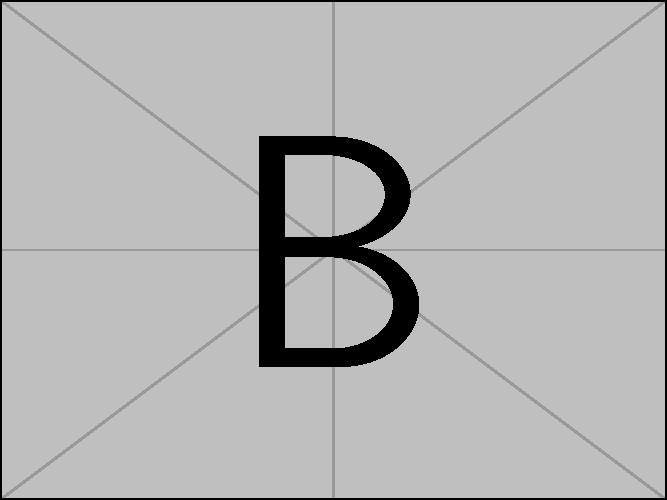
\includegraphics[width=0.45\linewidth]{example-image-b.pdf}}
  \caption{多个分图的示例}
  \label{fig:multi-image}
\end{figure}



\section{表格}

表应具有自明性。为使表格简洁易读,尽可能采用三线表,如表~\ref{tab:three-line}。
三条线可以使用 \pkg{booktabs} 宏包提供的命令生成。

\begin{table}
  \centering
  \caption{三线表示例}
  \begin{tabular}{ll}
    \toprule
    文件名          & 描述                         \\
    \midrule
    thuthesis.dtx   & 模板的源文件,包括文档和注释 \\
    thuthesis.cls   & 模板文件                     \\
    thuthesis-*.bst & BibTeX 参考文献表样式文件    \\
    thuthesis-*.bbx & BibLaTeX 参考文献表样式文件  \\
    thuthesis-*.cbx & BibLaTeX 引用样式文件        \\
    \bottomrule
  \end{tabular}
  \label{tab:three-line}
\end{table}

表格如果有附注,尤其是需要在表格中进行标注时,可以使用 \pkg{threeparttable} 宏包。
研究生要求使用英文小写字母 a、b、c……顺序编号,本科生使用圈码 ①、②、③……编号。

\begin{table}
  \centering
  \begin{threeparttable}[c]
    \caption{带附注的表格示例}
    \label{tab:three-part-table}
    \begin{tabular}{ll}
      \toprule
      文件名                 & 描述                         \\
      \midrule
      thuthesis.dtx\tnote{a} & 模板的源文件,包括文档和注释 \\
      thuthesis.cls\tnote{b} & 模板文件                     \\
      thuthesis-*.bst        & BibTeX 参考文献表样式文件    \\
      thuthesis-*.bbx        & BibLaTeX 参考文献表样式文件  \\
      thuthesis-*.cbx        & BibLaTeX 引用样式文件        \\
      \bottomrule
    \end{tabular}
    \begin{tablenotes}
      \item [a] 可以通过 xelatex 编译生成模板的使用说明文档;
        使用 xetex 编译 \file{thuthesis.ins} 时则会从 \file{.dtx} 中去除掉文档和注释,得到精简的 \file{.cls} 文件。
      \item [b] 更新模板时,一定要记得编译生成 \file{.cls} 文件,否则编译论文时载入的依然是旧版的模板。
    \end{tablenotes}
  \end{threeparttable}
\end{table}

% !TeX root = ../thuthesis-example.tex

\chapter{数学符号和公式}

\section{数学符号}

研究生《写作指南》要求量及其单位所使用的符号应符合国家标准《国际单位制及其应用》(GB 3100—1993)、《有关量、单位和符号的一般原则》(GB/T 3101—1993) 的规定。
模板中使用 \pkg{unicode-math} 宏包来配置数学符号,
与 \LaTeX{} 默认的英美国家的符号习惯有所差异:
\begin{enumerate}
  \item 大写希腊字母默认为斜体,如 \cs{Delta}:$\Delta$。
  \item 有限增量符号 $\increment$(U+2206)应使用 \pkg{unicode-math} 宏包提供的
    \cs{increment} 命令。
  \item 向量、矩阵和张量要求粗斜体,应该使用 \pkg{unicode-math} 的 \cs{symbf} 命令,
    如 \verb|\symbf{A}|、\verb|\symbf{\alpha}|。
  \item 数学常数和特殊函数要求用正体,应使用 \cs{symup} 命令,
    如 $\symup{\pi} = 3.14\dots$; $\symup{e} = 2.718\dots$,
  \item 微分号和积分号使用使用正体,比如 $\int f(x) \dif x$。
\end{enumerate}

关于数学符号更多的用法,参考
\href{http://mirrors.ctan.org/macros/latex/contrib/unicode-math/unicode-math.pdf}{\pkg{unicode-math}}
宏包的使用说明,
全部数学符号命的令参考
\href{http://mirrors.ctan.org/macros/latex/contrib/unicode-math/unimath-symbols.pdf}{\pkg{unimath-symbols}}。

关于量和单位推荐使用
\href{http://mirrors.ctan.org/macros/latex/contrib/siunitx/siunitx.pdf}{\pkg{siunitx}}
宏包,
可以方便地处理希腊字母以及数字与单位之间的空白,
比如:
\SI{6.4e6}{m},
\SI{9}{\micro\meter},
\si{kg.m.s^{-1}},
\SIrange{10}{20}{\degreeCelsius}。



\section{数学公式}

数学公式可以使用 \env{equation} 和 \env{equation*} 环境。
注意数学公式的引用应前后带括号,建议使用 \cs{eqref} 命令,比如式 \eqref{eq:example}。
\begin{equation}
  \frac{1}{2 \symup{\pi} \symup{i}} \int_\gamma f = \sum_{k=1}^m n(\gamma; a_k) \mathscr{R}(f; a_k)
  \label{eq:example}
\end{equation}
注意公式编号的引用应含有圆括号,可以使用 \cs{eqref} 命令。

多行公式尽可能在“=”处对齐,推荐使用 \env{align} 环境。
\begin{align}
  a & = b + c + d + e \\
    & = f + g
\end{align}



\section{数学定理}

定理环境的格式可以使用 \pkg{amsthm} 或者 \pkg{ntheorem} 宏包配置。
用户在导言区载入这两者之一后,模板会自动配置 \env{thoerem}、\env{proof} 等环境。

\begin{theorem}[Lindeberg--Lévy 中心极限定理]
  设随机变量 $X_1, X_2, \dots, X_n$ 独立同分布, 且具有期望 $\mu$ 和有限的方差 $\sigma^2 \ne 0$,
  记 $\bar{X}_n = \frac{1}{n} \sum_{i+1}^n X_i$,则
  \begin{equation}
    \lim_{n \to \infty} P \left(\frac{\sqrt{n} \left( \bar{X}_n - \mu \right)}{\sigma} \le z \right) = \Phi(z),
  \end{equation}
  其中 $\Phi(z)$ 是标准正态分布的分布函数。
\end{theorem}
\begin{proof}
  Trivial.
\end{proof}

同时模板还提供了 \env{assumption}、\env{definition}、\env{proposition}、
\env{lemma}、\env{theorem}、\env{axiom}、\env{corollary}、\env{exercise}、
\env{example}、\env{remar}、\env{problem}、\env{conjecture} 这些相关的环境。

% !TeX root = ../thuthesis-example.tex

\chapter{实验分析与方法应用}

\section{引言}
\label{exp.intro}

本文提出了一种专门适用于细粒度领域适应问题的领域适应方法——渐进对抗网络。
为客观可靠评价本文所提出的渐进对抗网络的有效性,需要对算法进行实现,并开展对比实验和分析实验。
由于公开数据集缺乏,本文自行搜集数据、构建了两个细粒度领域适应数据集。
另外,为降低用户使用门槛,本文将算法集成到了领域适应学习系统中,并实现了在实际任务中的应用。

本节中将介绍渐进对抗网络实现方案、所选用的对比算法、评价算法性能所采用的指标、以及分析实验的设定。


% % \textbf{本章内容安排。}本章主要内容是实验分析与方法应用,共含有7节。除第\ref{exp.intro}节引言以外,其余6节的内容安排如下:
% % \begin{itemize}
% % \item 第\ref{exp.setting}节是实验设置,由4个小节构成。
% % 其一,介绍本文实现渐进对抗网络所选用的深度学习框架;
% % 其二,介绍本文实验运行的环境;
% % 其三,介绍模型训练中的各项设定;
% % 最后,介绍本文评价模型性能优劣所采用的评价指标。
% % \item 第\ref{exp.dataset}节是数据集构建,由2个小节构成。分别介绍,从采集清洗数据开始,构建两个专门的细粒度领域适应数据集Birds-31和CUB-Paintings的过程。
% % \item 第\ref{exp.result}节是对比实验,在本章构建的数据集上,将渐进对抗网络与最新的领域适应方法和图像识别方法进行对比,并对实验现象背后的原因进行分析。
% % \item 第\ref{exp.analyse}节是分析实验,设计了若干分析实验,对渐进对抗网络各个部分的设计动机,以及渐进对抗网络所提取特征的迁移性能和判别性能进行分析。
% % \item 第\ref{exp.application}节是应用案例,对将渐进对抗网络与大数据系统软件国家工程实验室领域适应学习系统Xlearn-DA的集成过程进行介绍,对渐进对抗网络在监控视频车辆品牌型号识别任务上的应用进行介绍。
% % \item 第\ref{exp.last}节是本章小结,尝试对本章中包含的各项工作加以总结概括。
% % \end{itemize}




% \section{实验设置}
% \label{exp.setting}

\subsection{深度学习框架}
近年来,随着深度学习的蓬勃发展,学术界和工业界对深度学习研究的投入不断扩大,催生了许多深度学习框架,比如Caffe\cite{jia2014caffe}、Tensorflow\cite{abadi2016tensorflow}、MXNet\cite{chen2015mxnet}和Pytorch\cite{paszke2019pytorch}。
这些深度学习框架各具特点、各擅胜场。

但是,目前,在学术界,Pytorch被越来越多的研究人员采用,已经有逐渐成为主流的趋势。
为便于模型实现、利于同行间交流,本文采用深度学习框架Pytorch来实现本文提出的渐进对抗网络。
详细的网络设计见于第章。

\subsection{实验环境}
本文实验在装备图形处理器(Graphics Processing Unit,GPU)的深度学习服务器上进行。
该服务器配备有8块型号为NVIDIA TITAN RTX的图形处理器,具体配置参见表。
该型号的图形处理器采用Turing架构,具有24GB显存。
较大的显存给模型的训练带来极大的便利。因为在渐进对抗网络中,辅助的粗粒度特征提取器和细粒度特征提取器并不共享参数。所以,在训练阶段,渐进对抗网络所需显存大小大约为一般卷积神经网络的两倍。
当然,深度学习框架支持将单一模型分配到多块图形处理器上进行训练,只是可能造成训练速度的下降。

其实,近年来深度学习的快速发展离不开计算机硬件性能的不断提升,尤其是图形处理器性能的不断提升。
相较于擅长处理涉及复杂计算步骤、涉及复杂数据依赖的计算任务的中央处理器(Central Processing Unit,CPU),众核架构的图形处理器更适合处理密集计算、并行计算。
在深度网络训练这一特别任务上,图形处理器表现远远优于中央处理器,此二者的性能差异可能高达数十倍。
性能屡创新高的图形处理器,使得利用海量数据训练深达上千层的深度神经网络成为可能。
此外,NVIDIA公司数十年来对于底层库通用并行计算架构(Compute Unified Device Architecture,CUDA)和深度神经网络图形处理器加速器(NVIDIA CUDA Deep Neural Network library,NVIDIA cuDNN)的不断优化,也构成了深度学习领域研究不断前进的基础。

% % 当然,近年来,工业界不断有新的力量被投入参与深度学习硬件的设计开发,比如谷歌公司(Google)研发的机器学习定制芯片——张量处理器(Tensor Processing Unit,TPU)。
% % 这些持续不断的投入极大的促进了深度学习的繁荣。


% \newcolumntype{Y}{>{\centering\arraybackslash}X} 
% \begin{table}[htb]
%   \centering
%   \caption[模板文件]{服务器配置}
%   \label{tab:gpu}
%     \begin{tabular}{\linewidth}{lc}
%       \toprule
%       {\heiti 项目} & {\heiti 配置信息} \\\midrule[1pt]
%       操作系统 & Ubuntu 18.04.3 LTS \\
%       中央处理器 & Intel(R) Xeon(R) Gold 6130 CPU @ 2.10GHz \\
%       中央处理器核数 & 64 \\
%       内存    & 512GB \\
%       图形处理器    & NVIDIA TITAN RTX \\
%       显存   & 24GB \\
%       Pytorch版本   & 0.4.1 \\
%       CUDA版本   & 10.2 \\
%       \bottomrule
%     \end{tabular}
% \end{table}

\begin{table}
  \centering
  \caption{服务器配置}
  \begin{tabular}{lc}
    \toprule
    项目  & 配置信息       \\
    \midrule
    操作系统 & Ubuntu 18.04.3 LTS \\
    中央处理器 & Intel(R) Xeon(R) Gold 6130 CPU @ 2.10GHz \\
    中央处理器核数 & 64 \\
    内存    & 512GB \\
    图形处理器    & NVIDIA TITAN RTX \\
    显存   & 24GB \\
    PyTorch版本   & 0.4.1 \\
    CUDA版本   & 10.2 \\
    \bottomrule
  \end{tabular}
  \label{tab:gpu}
\end{table}


% % \subsection{模型训练}
% % 本文使用深度学习框架PyTorch\cite{paszke2019pytorch}实现所提出的渐进对抗网络。
% % 粗粒度特征提取器$\rm G$和细粒度特征提取器$\rm F$是移除最后一层分类器层后的ResNet-50\cite{he2016deep}网络。也就是说,本文采用的基干网络(Backbone)是ResNet-50。
% % ResNet-50网络将首先在ImageNet\cite{russakovsky2015imagenet}上进行预训练,之后,在训练过程中,在我们的数据集上进行微调(Fine-tune)。
% % 而粗粒度类别预测器${\rm C}^k |_{k=1}^K$、细粒度类别预测器$\rm Y$和领域判别器$\rm D$是随机初始化参数后进行训练的。

% % 本文采用小批量随机梯度下降方法(Mini-batch Stochastic Gradient Desent,Mini-batch SGD),在图形处理器NVIDIA TITAN RTX上,对网络进行训练。动量(Momentum)设置为0.9,批量大小(Batch Size)设置为36。
% % 在网络训练过程中,参数随机初始化后进行训练的网络的学习率被设置为预训练-微调部分网络的学习率的10倍。
% % 分类损失函数和对抗损失函数的权重$\lambda$采用变化策略$\lambda=\frac{1-exp⁡(-10p)}{1+exp(-10p)}$,这是被对抗领域适应方法最广泛采用的。
% % 本文并没有针对各个迁移学习任务调整超参数,在所有的迁移学习任务上,这些参数都是保持一致的。


% % \subsection{评价指标}
% % 本文所研究的问题——细粒度领域适应,是无监督的。
% % 这意味着,在训练过程中,目标领域样本的类别信息是不可见的。
% % 与一般的无监督领域适应问题一致,本文采用模型在目标域上的样本分类准确率作为评价模型性能的主要指标。

% % 具体来说,目标领域样本分类准确率通过这样的方法来计算。
% % 在训练过程中,我们将被给定一个拥有$n_{\mathcal{S}}$个样本的源领域$\mathcal{S} = \{({x},{y}_f,{y}_c^k|_{k=1}^K)\}$ ,和一个拥有$n_{\mathcal{T}}$个样本的目标领域${{\mathcal{T}}} = \{({x}, \textrm{?}, \textrm{?} )\}$。
% % 在预测过程中,我们将被给定$n_{\mathcal{T}}$个带有标签的目标领域样本对$({x},{y}_f)$,我们将利用已经训练好的细粒度特征提取器$\rm F$和类别预测器$\rm Y$对目标领域$\mathcal{T}$上的这$n_{\mathcal{T}}$个样本的细粒度类别进行预测,$\hat{y}_f={\rm Y}\left({\rm F}\left(x\right)\right)$。
% % % 在评价模型性能的时候,我们将获得目标域$\mathcal{T}$上的样本的标记信息${y_f}$。
% % 最后,统计所有样本$x$的预测标签$\hat{y}_f$和真实标签$y_f$是否一致,计算模型预测的细粒度类别准确率,评价模型的优劣:
% % \begin{equation}
% % % acc = \frac{ \sum\limits_{{x} \in {\mathcal{S}}}  \mathbb{I}\left(  {\rm Y}\left({\rm F}\left(x\right)\right)  = y_f \right)}{n_{\mathcal{T}}},
% % acc = { \sum\limits_{{x} \in {\mathcal{T}}}  \mathbb{I}\left(  {\rm Y}\left({\rm F}\left(x\right)\right)  , y_f \right)}/{n_{\mathcal{T}}},
% % \end{equation}
% % 其中,$ \mathbb{I}$是指示函数,一致则取1,不一致则取0:
% % \begin{equation}
% %   \mathbb{I}\left(  {\rm Y}\left({\rm F}\left(x\right)\right), y_f \right) = 
% %   \begin{cases}
% %     1, \quad {\rm Y}\left({\rm F}\left(x\right)\right)  = y_f; \\[0.1cm]
% %     0, \quad  {\rm Y}\left({\rm F}\left(x\right)\right) \neq y_f.
% %   \end{cases}
% % \end{equation}


% % \section{数据集构建}
% % \label{exp.dataset}
% % 细粒度领域适应是领域适应问题的一个细分研究方向,专门数据集缺乏。近年来,无论是细粒度视觉识别还是领域适应,均吸引了越来越多的关注。随着研究热度的提升,支持细粒度视觉识别和领域适应这两个问题的研究的基础设置愈加完善。最直接的表现就是,用于评价细粒度视觉识别算法和领域适应算法的数据集种类不断丰富、数量不断扩大。新的细粒度视觉识别数据集不断涌现,覆盖的物体种类范围越来越广。鸟\cite{welinder2010caltech,wah2011caltech,NABirds},狗\cite{standforddog,liu2012dog},花\cite{nilsback2006flower,angelova2013flower},飞机\cite{vedaldi2014air,maji2013air},汽车\cite{stark2011car,krause20133dcar,lin2014jointlycar,yang2015largecar}和食物 \cite{bossard2014food}都有专门的数据集。但是,专门为细粒度领域适应问题搜集建立的数据集尚属极少数。缺乏专门用于细粒度领域适应问题的公开数据集严重制约了对这一极具挑战性、极具学术研究价值的问题的深入研究。


% % 于是,为了能够对本文所提出的专门用于细粒度场景的领域适应方法——渐进对抗网络进行客观的、充分的评价,为了能够尽己所能推动细粒度领域适应问题的研究,本文尝试搜集和构建了两个专门用于细粒度领域适应的数据集:Birds-31和CUB-Paintings。
% % 数据集Birds-31基于三个被广泛使用的细粒度视觉识别数据集构建。三个数据集天然构成了迁移学习的三个领域。
% % 但是,数据集Birds-31领域间差异过小,不能对领域适应方法进行充分的检验。
% % 所以,本文从互联网上爬取了大量图像数据并进行了人工筛选,构建了数据集CUB-Paintings。
% % 本文所构建的两个数据集的概况(所含领域、各个领域所含样本数量)见于下表\ref{table.imagenum}中。
% % \begin{table}[htbp]
% % \addtolength{\tabcolsep}{15pt}
% % \caption[模板文件]{数据集概况}
% % \vspace{-15pt}
% % \begin{center}
% % %  \begin{minipage}[t]{0.8\linewidth} % 如果想在表格中使用脚注,minipage是个不错的办法
% % \begin{tabular}{l|c|c}
% % \toprule[1.5pt]
% %  {\heiti 数据集}& {\heiti 领域}& {\heiti 图像数量}\\
% % \midrule
% % \multirow{3}*{{Birds-31}} & \multicolumn{1}{c|}{CUB-200-2011} & \multicolumn{1}{c}{1848}\\
% % & NABirds & 2988 \\
% % & iNaturalist2017 & 2857 \\
% % \midrule
% % \multirow{2}*{{CUB-Paintings}} & \multicolumn{1}{c|}{CUB-200-2011} & \multicolumn{1}{c}{11788}\\
% % & CUB-200-Painting & 3047 \\


% % \bottomrule[1.5pt]
% % \end{tabular}
% % \end{center}
% % \label{table.imagenum}
% % \vspace{-10pt}
% % \end{table}



% % \iffalse
% % \newcolumntype{Y}{>{\centering\arraybackslash}X} 
% % \begin{table}[htb]
% %   \centering
% %   \begin{minipage}[t]{0.8\linewidth} % 如果想在表格中使用脚注,minipage是个不错的办法
% %   \caption[模板文件]{服务器配置}
% %   \label{tab:gpu}
% %     \begin{tabularx}{\linewidth}{lYY}
% %      \toprule[1.5pt]
% % 	数据集&领域&图像数量\\
% % 	\midrule
% % 	\multirow{2}*{{CUB-Paintings}} & \multicolumn{1}{c|}{CUB-200-2011} & \multicolumn{1}{c}{11788}\\
% % 	& CUB-200-Painting & 3047 \\
% % 	\midrule
% % 	\multirow{3}*{{Birds-31}} & \multicolumn{1}{c|}{CUB-200-2011} & \multicolumn{1}{c}{1848}\\
% % 	& NABirds & 2988 \\
% % 	& iNaturalist2017 & 2857 \\
% % 	\bottomrule[1.5pt]
% %     \end{tabularx}
% %   \end{minipage}
% % \end{table}




% % \newcolumntype{Y}{>{\centering\arraybackslash}X} 
% % \begin{table}[htb]
% %   \centering
% %   \begin{minipage}[t]{0.8\linewidth} % 如果想在表格中使用脚注,minipage是个不错的办法
% %   \caption[模板文件]{服务器配置}
% %   \label{tab:gpu}
% %     \begin{tabularx}{\linewidth}{lY}
% %       \toprule[1.5pt]
% %       {\heiti 项目} & {\heiti 配置信息} \\\midrule[1pt]
% %       操作系统 & Ubuntu 18.04.3 LTS \\
% %       中央处理器 & Intel(R) Xeon(R) Gold 6130 CPU @ 2.10GHz \\
% %       中央处理器核数 & 64 \\
% %       内存    & 512GB \\
% %       图形处理器    & NVIDIA TITAN RTX \\
% %       显存   & 24GB \\
% %       Pytorch版本   & 0.4.1 \\
% %       CUDA版本   & 10.2 \\
% %       \bottomrule[1.5pt]
% %     \end{tabularx}
% %   \end{minipage}
% % \end{table}


% 其他部分
\backmatter

% 参考文献
\bibliography{ref/refs}  % 参考文献使用 BibTeX 编译
% \printbibliography       % 参考文献使用 BibLaTeX 编译

% 附录
\appendix
\chapter{补充内容}

附录是与论文内容密切相关、但编入正文又影响整篇论文编排的条理和逻辑性的资料,例如某些重要的数据表格、计算程序、统计表等,是论文主体的补充内容,可根据需要设置。


\section{图表示例}

\subsection{图}

附录中的图片示例(图~\ref{fig:appendix-figure})。

\begin{figure}[ht]
  \centering
  
\includegraphics[width=0.6\linewidth]{example-image-a.pdf}
  \caption{附录中的图片示例}
  \label{fig:appendix-figure}
\end{figure}


\subsection{表格}

附录中的表格示例(表~\ref{tab:appendix-table})。

\begin{table}[ht]
  \centering
  \caption{附录中的表格示例}
  \begin{tabular}{ll}
    \toprule
    文件名          & 描述                         \\
    \midrule
    thuthesis.dtx   & 模板的源文件,包括文档和注释 \\
    thuthesis.cls   & 模板文件                     \\
    thuthesis-*.bst & BibTeX 参考文献表样式文件    \\
    thuthesis-*.bbx & BibLaTeX 参考文献表样式文件  \\
    thuthesis-*.cbx & BibLaTeX 引用样式文件        \\
    \bottomrule
  \end{tabular}
  \label{tab:appendix-table}
\end{table}


\section{数学公式}

附录中的数学公式示例(公式~\eqref{eq:appendix-equation})。
\begin{equation}
  \frac{1}{2 \symup{\pi} \symup{i}} \int_\gamma f = \sum_{k=1}^m n(\gamma; a_k) \mathscr{R}(f; a_k)
  \label{eq:appendix-equation}
\end{equation}

% % !TeX root = ../thuthesis-example.tex

\begin{survey}
\label{cha:survey}

\title{Title of the Survey}
\maketitle


\tableofcontents


本科生的外文资料调研阅读报告。


\section{Figures and Tables}

\subsection{Figures}

An example figure in appendix (Figure~\ref{fig:appendix-survey-figure}).

\begin{figure}
  \centering
  
\includegraphics[width=0.6\linewidth]{example-image-a.pdf}
  \caption{Example figure in appendix}
  \label{fig:appendix-survey-figure}
\end{figure}


\subsection{Tables}

An example table in appendix (Table~\ref{tab:appendix-survey-table}).

\begin{table}
  \centering
  \caption{Example table in appendix}
  \begin{tabular}{ll}
    \toprule
    File name       & Description                                         \\
    \midrule
    thuthesis.dtx   & The source file including documentaion and comments \\
    thuthesis.cls   & The template file                                   \\
    thuthesis-*.bst & BibTeX styles                                       \\
    thuthesis-*.bbx & BibLaTeX styles for bibliographies                  \\
    thuthesis-*.cbx & BibLaTeX styles for citations                       \\
    \bottomrule
  \end{tabular}
  \label{tab:appendix-survey-table}
\end{table}


\section{Equations}

An example equation in appendix (Equation~\eqref{eq:appendix-survey-equation}).
\begin{equation}
  \frac{1}{2 \symup{\pi} \symup{i}} \int_\gamma f = \sum_{k=1}^m n(\gamma; a_k) \mathscr{R}(f; a_k)
  \label{eq:appendix-survey-equation}
\end{equation}


\section{Citations}

Example citations in appendix.
\cite{abrahams99tex}
\cite{salomon1995advanced}
\cite{abrahams99tex,salomon1995advanced}


\bibliographystyle{unsrtnat}
\bibliography{ref/appendix}

\end{survey}
       % 本科生:外文资料的调研阅读报告
% % !TeX root = ../thuthesis-example.tex

\begin{translation}
\label{cha:translation}

\title{书面翻译题目}
\maketitle

\tableofcontents


本科生的外文资料书面翻译。


\section{图表示例}

\subsection{图}

附录中的图片示例(图~\ref{fig:appendix-translation-figure})。

\begin{figure}
  \centering
  
\includegraphics[width=0.6\linewidth]{example-image-a.pdf}
  \caption{附录中的图片示例}
  \label{fig:appendix-translation-figure}
\end{figure}


\subsection{表格}

附录中的表格示例(表~\ref{tab:appendix-translation-table})。

\begin{table}
  \centering
  \caption{附录中的表格示例}
  \begin{tabular}{ll}
    \toprule
    文件名          & 描述                         \\
    \midrule
    thuthesis.dtx   & 模板的源文件,包括文档和注释 \\
    thuthesis.cls   & 模板文件                     \\
    thuthesis-*.bst & BibTeX 参考文献表样式文件    \\
    thuthesis-*.bbx & BibLaTeX 参考文献表样式文件  \\
    thuthesis-*.cbx & BibLaTeX 引用样式文件        \\
    \bottomrule
  \end{tabular}
  \label{tab:appendix-translation-table}
\end{table}


\section{数学公式}

附录中的数学公式示例(公式~\eqref{eq:appendix-translation-equation})。
\begin{equation}
  \frac{1}{2 \symup{\pi} \symup{i}} \int_\gamma f = \sum_{k=1}^m n(\gamma; a_k) \mathscr{R}(f; a_k)
  \label{eq:appendix-translation-equation}
\end{equation}


\section{文献引用}

文献引用示例\cite{abrahams99tex}。


% 书面翻译的参考文献
\bibliographystyle{unsrtnat}
\bibliography{ref/appendix}

% 书面翻译对应的原文索引
\begin{translation-index}
  \nocite{salomon1995advanced}
  \bibliographystyle{unsrtnat}
  \bibliography{ref/appendix}
\end{translation-index}

\end{translation}
  % 本科生:外文资料的书面翻译

% 致谢
% !TeX root = ../thuthesis-example.tex

\begin{acknowledgements}
  衷心感谢导师×××教授和物理系××副教授对本人的精心指导。他们的言传身教将使我终生受益。

  在美国麻省理工学院化学系进行九个月的合作研究期间,承蒙 Robert Field 教授热心指导与帮助,不胜感激。

  感谢×××××实验室主任×××教授,以及实验室全体老师和同窗们学的热情帮助和支持!

  本课题承蒙国家自然科学基金资助,特此致谢。
\end{acknowledgements}


% 声明
\statement
% 生成的声明页是否要插入页眉和页脚(默认 empty)
% 仅在需要进行电子签名时,才需要打开这一选项
% 插入的扫描声明页总是会生成页眉(研究生)和页脚,不受这一选项影响
% \statement[page-style=plain]
% 将签字扫描后的声明文件 scan-statement.pdf 替换原始页面
% \statement[file=scan-statement.pdf]

% 个人简历、在学期间完成的相关学术成果
% !TeX root = ../thuthesis-example.tex

\begin{resume}

  \section*{个人简历}

  1995年11月21日出生于内蒙古包头市九原区。

  2014年8月考入北京航空航天大学软件工程专业,曾获得国家奖学金,国家励志奖学金等。2018年7月本科毕业并获得工学学士学位。

  2018年8月推荐免试进入清华大学软件学院攻读工程硕士学位至今,2020年6月至2021年3月在腾讯人工智能实验室联合培养。曾获国家奖学金,英特尔奖学金等。


  \section*{在学期间完成的相关学术成果}

  \subsection*{学术论文}

  \begin{achievements}
    \item Xinyang Chen, Sinan Wang, \textbf{Bo Fu}, Mingsheng Long, Jianmin Wang. Catastrophic Forgetting Meets Negative Transfer: Batch Spectral Shrinkage for Safe Transfer Learning [C]. Advances in Neural Information Processing Systems, NeurIPS, 2019: 1906-1916. (Regular Paper,CCF A类会议,EI会议)
    \item \textbf{Bo Fu}, Zhangjie Cao, Mingsheng Long, Jianmin Wang. Learning to Detect Open Classes for Universal Domain Adaptation [C]. European Conference on Computer Vision, ECCV, 2020: 567-583.  (Regular Paper,CCF B类会议,EI会议)
    \item \textbf{Bo Fu}, Zhangjie Cao, Mingsheng Long, Jianmin Wang. Transferable Query Selection for Active Domain Adaptation [C]. IEEE Conference on Computer Vision and Pattern Recognition, CVPR, 2021.  (Regular Paper,CCF A类会议,EI会议)
  \end{achievements}

%   \begin{publications}
%     \item Xinyang Chen , Sinan Wang , Bo Fu, Mingsheng Long, Jianmin Wang. Catastrophic Forgetting Meets Negative Transfer: Batch Spectral Shrinkage for Safe Transfer Learning. Advances in Neural Information Processing Systems,NeurIPS 2019: 1906-1916. (Regular Paper,CCF A类会议,EI会议)
%   \end{publications}

%  \begin{publications}[before=\publicationskip,after=\publicationskip]
%     \item  \textbf{Sinan Wang}, Xinyang Chen, Yunbo Wang, Mingsheng Long, Jianmin Wang. Progressive Adversarial Networks for Fine-Grained Domain Adaptation. Accepted by 2020 IEEE Conference on Computer Vision and Pattern Recognition,CVPR 2020. (Regular Paper,CCF A类会议,EI会议)
%   \end{publications}
  
%   \begin{publications}
%     \item Xinyang Chen, \textbf{Sinan Wang}, Mingsheng Long, Jianmin Wang. Transferability vs. Discriminability: Batch spectral penalization for adversarial domain adaptation. Proceedings of the 36th International Conference on Machine Learning,ICML 2019: 1081-1090. (Regular Paper,CCF A类会议,EI收录,检索号: 20200408068065)
%   \end{publications}


  \subsection*{专利}

  \begin{achievements}
    \item 王建民, 龙明盛, 付博, 黄向东. 一种机器学习算法自动选择方法和系统: 中国, CN108009643B[P]. 2018-10-30.
    \item 王建民, 龙明盛, 付博, 黄向东. 一种大数据分析开发平台中异构算子管理方法: 中国, CN107943945B[P]. 2018-12-11.
  \end{achievements}

  \subsection*{开源项目}
  \begin{achievements}
    \item Junguang Jiang, Bo Fu, Mingsheng Long. Transfer-Learning-library [CP/OL]. [2020-08-04]. https://github.com/thuml/Transfer-Learning-Library 
  \end{achievements}
  
\end{resume}


% 指导教师/指导小组学术评语
% !TeX root = ../thuthesis-example.tex

\chapter{指导小组学术评语}

论文提出了……


% 答辩委员会决议书
% !TeX root = ../thuthesis-example.tex

\chapter{答辩委员会决议书}

论文提出了……

论文取得的主要创新性成果包括:

1. ……

2. ……

3. ……

论文工作表明作者在×××××具有×××××知识,具有××××能力,论文××××,答辩××××。

答辩委员会表决,(×票/一致)同意通过论文答辩,并建议授予×××(姓名)×××(门类)学博士/硕士学位。


% 本科生的综合论文训练记录表(扫描版)
% \record{file=scan-record.pdf}

\end{document}
